% =====================================================================
%  gTAO-Net Article 2, IEEE Access version (built from paper/sections, 2026-11-23).
%  Numbers come from ../tables (generated); do not type numbers by hand.
%  Uses the official ieeeaccess.cls when it is present in this folder,
%  otherwise IEEEtran (same structure, for drafting only).
%  Build: latexmk -pdf main.tex
% =====================================================================
\IfFileExists{ieeeaccess.cls}{\documentclass{ieeeaccess}\newif\ifaccess\accesstrue}{\documentclass[journal]{IEEEtran}\newif\ifaccess\accessfalse}
\usepackage[T1]{fontenc}
\usepackage[utf8]{inputenc}
\usepackage{cite}
\usepackage{amsmath,amssymb}
\usepackage{booktabs}
\usepackage{array}
\usepackage{graphicx}
\usepackage{xcolor}
% The architecture figure is pre-rendered (figsrc/fig_arch.tex): ieeeaccess.cls conflicts with TikZ.
\usepackage{xurl}
\usepackage[hidelinks]{hyperref}

\newcommand{\qwk}{QWK}
\newcommand{\pending}[1]{\textcolor{red}{\textbf{[#1]}}}
\newif\ifnested
\nestedtrue

\newif\ifcmptest
\newcommand{\cmpBestName}{face stream, CORAL}
\newcommand{\cmpBestQWK}{0.043}
\newcommand{\cmpBestQWKsd}{0.013}
\newcommand{\cmpBestAcc}{50.4}
\newcommand{\cmpMajAcc}{51.8}
\newcommand{\cmpNScored}{1{,}638}
\cmptesttrue

\input{tables/fullcorpus_numbers}

\ifaccess\else
  \newenvironment{keywords}{\begin{IEEEkeywords}}{\end{IEEEkeywords}}
  \providecommand{\PARstart}[2]{\IEEEPARstart{#1}{#2}}
  \providecommand{\EOD}{}
\fi

\begin{document}
\ifaccess
\history{Date of publication xxxx 00, 0000, date of current version xxxx 00, 0000.}
\doi{10.1109/ACCESS.2026.DOI}
% Previous (fusion-first) title: Does Multimodal Fusion Help Classroom Attention Estimation? A Controlled Diagnostic of Gated Ordinal Fusion on DIPSER, DAiSEE and EngageNet
\title{The Evaluation Protocol Outweighs Fusion in Classroom Attention Estimation: A Controlled Study on DIPSER, DAiSEE and EngageNet}
\author{\uppercase{Zakaria Makhkhas}\authorrefmark{1}, \uppercase{Amal Rifai}\authorrefmark{2}, and \uppercase{Abdelalim Sadiq}\authorrefmark{1}}
\address[1]{Laboratory of Information Modelling and Communication Systems, Faculty of Sciences, University Ibn Tofail, K\'enitra, Morocco}
\address[2]{Team of Research in Engineering of Computing Environment for Human Learning, Regional Center for the Professions of Education and Training (RCPET), Rabat, Morocco}
\tfootnote{This research did not receive any specific grant from funding agencies in the public, commercial, or not-for-profit sectors.}
\markboth{Makhkhas \headeretal: The Evaluation Protocol Outweighs Fusion in Classroom Attention Estimation}{Makhkhas \headeretal: The Evaluation Protocol Outweighs Fusion in Classroom Attention Estimation}
\corresp{Corresponding author: Zakaria Makhkhas (e-mail: zakaria.makhkhas@uit.ac.ma).}
\begin{abstract}
Multimodal attention systems assume that fusing more data streams improves recognition. We test this with gTAO-Net, one model in which each design choice is a switch: gated versus mean-pooled fusion, a linear input-to-head link, modality dropout, and three ordinal objectives (CORAL, a CORE-style hybrid and a soft multi-rater target). All streams share a training-free Tchebichef-moment front-end. On a DIPSER slice of 20 students, none of the 24 fusion configurations exceeds the best single stream (face mesh with the soft target, QWK $0.256\pm0.068$, against $0.124\pm0.071$ for the best fusion), and the gate is not significantly different from mean pooling ($p=0.68$). Only the input-to-head link ($p=0.002$) and the soft target ($p=0.023$) help, and fusion yields no meaningful gain on DAiSEE or EngageNet. On the full DIPSER release (\fcPersons{} students, \fcWindows{} windows) the fusion result replicates (\fcFusionsAbove{} fusions above it), but the sensor signal is weak (best QWK \fcBestSingleQWK) and largely shared by the class. Hyper-parameter search, richer and local moments, a face crop, frozen pretrained face encoders, and temporal and class context do not improve on it. A label probe every 32\,s raises accuracy to \fcProbeHalfAcc\% on an unseen class, but repeating the probe already gives \fcPersistHalfAcc\%. The evaluation protocol has a larger effect than any of these choices: the same model obtains QWK \fcLeakRandQWK{} on random windows, \fcLeakPersonQWK{} on held-out students and \fcLogoOwnQWK{} on a held-out class, while its accuracy remains close to the majority rate (\fcMajority\%).
\end{abstract}

\begin{keywords}
Data leakage, DIPSER, evaluation protocol, multimodal fusion, multi-rater labels, ordinal regression, student attention, Tchebichef moments.
\end{keywords}

\titlepgskip=-15pt
\maketitle
\else
% Previous (fusion-first) title: Does Multimodal Fusion Help Classroom Attention Estimation? A Controlled Diagnostic of Gated Ordinal Fusion on DIPSER, DAiSEE and EngageNet
\title{The Evaluation Protocol Outweighs Fusion in Classroom Attention Estimation: A Controlled Study on DIPSER, DAiSEE and EngageNet}
\author{Zakaria Makhkhas, Amal Rifai, and Abdelalim Sadiq%
\thanks{Z. Makhkhas and A. Sadiq are with the Laboratory of Information Modelling and Communication Systems, Faculty of Sciences, University Ibn Tofail, K\'enitra, Morocco (e-mail: zakaria.makhkhas@uit.ac.ma).}%
\thanks{A. Rifai is with the Team of Research in Engineering of Computing Environment for Human Learning, Regional Center for the Professions of Education and Training (RCPET), Rabat, Morocco.}}
\markboth{Makhkhas \MakeLowercase{\textit{et al.}}: The Evaluation Protocol Outweighs Fusion in Classroom Attention Estimation}{}
\maketitle
\begin{abstract}
Multimodal attention systems assume that fusing more data streams improves recognition. We test this with gTAO-Net, one model in which each design choice is a switch: gated versus mean-pooled fusion, a linear input-to-head link, modality dropout, and three ordinal objectives (CORAL, a CORE-style hybrid and a soft multi-rater target). All streams share a training-free Tchebichef-moment front-end. On a DIPSER slice of 20 students, none of the 24 fusion configurations exceeds the best single stream (face mesh with the soft target, QWK $0.256\pm0.068$, against $0.124\pm0.071$ for the best fusion), and the gate is not significantly different from mean pooling ($p=0.68$). Only the input-to-head link ($p=0.002$) and the soft target ($p=0.023$) help, and fusion yields no meaningful gain on DAiSEE or EngageNet. On the full DIPSER release (\fcPersons{} students, \fcWindows{} windows) the fusion result replicates (\fcFusionsAbove{} fusions above it), but the sensor signal is weak (best QWK \fcBestSingleQWK) and largely shared by the class. Hyper-parameter search, richer and local moments, a face crop, frozen pretrained face encoders, and temporal and class context do not improve on it. A label probe every 32\,s raises accuracy to \fcProbeHalfAcc\% on an unseen class, but repeating the probe already gives \fcPersistHalfAcc\%. The evaluation protocol has a larger effect than any of these choices: the same model obtains QWK \fcLeakRandQWK{} on random windows, \fcLeakPersonQWK{} on held-out students and \fcLogoOwnQWK{} on a held-out class, while its accuracy remains close to the majority rate (\fcMajority\%).
\end{abstract}

\begin{keywords}
Data leakage, DIPSER, evaluation protocol, multimodal fusion, multi-rater labels, ordinal regression, student attention, Tchebichef moments.
\end{keywords}

\fi

\section{Introduction}
\label{sec:intro}

\PARstart{A}{utomatic} estimation of student engagement and attention has been studied for more than a decade, first from facial expressions~\cite{whitehill2014faces} and then from webcam recordings of individual learners such as DAiSEE~\cite{gupta2016daisee} and EngageNet~\cite{singh2023engagenet}. Recent systems combine several modalities (the face, facial landmarks, head pose and, when available, physiology) through attention or gating~\cite{baltrusaitis2019multimodal,arevalo2017gated,tran2026ordinal}, and data fusion is a recurrent theme of multimodal learning analytics~\cite{chango2022datafusionmmla}. The underlying premise is that each stream contributes information and that a learned fusion weights the streams appropriately.

This premise is rarely tested in isolation. Reported gains are usually accuracy differences on a single split, obtained with different backbones and protocols for the fused and the single-stream systems. The multimodal learning literature shows that a jointly trained model can underperform the best separately trained unimodal model, because the added capacity overfits and the modalities overfit and generalise at different rates~\cite{wang2020makes}, and because a dominant modality suppresses the optimisation of the others~\cite{peng2022balanced}. Engagement studies contain similar observations: the EngageNet baselines obtain a lower test accuracy with fused features than with one feature set~\cite{singh2023engagenet}, a study in secondary-school classrooms finds score-level fusion on par with the best modality~\cite{sumer2023multimodal}, and a recent transformer study on classroom data finds its fused model within the variability of its visual model~\cite{fragkiadakis2026fairness}. Whether fusion helps for classroom attention, where labels are noisy, ordinal and imbalanced, has nevertheless not been measured under a single controlled protocol.

A second, related question concerns the evaluation itself. Scores depend on what the test set shares with the training set, and such dependence is a documented cause of optimistic results in many fields~\cite{kapoor2023leakage}. In clinical and wearable sensing, splitting records rather than subjects is known to inflate performance~\cite{saeb2017need}, as does placing neighbouring windows on both sides of a split~\cite{hammerla2015lets}, and model-selection bias can be as large as the difference between learning algorithms~\cite{cawley2010overfitting}. Classroom data add a further level of structure: students of the same class attend the same lesson at the same time, so that windows of different students are not independent either.

DIPSER~\cite{marquezcarpintero2025dipser} makes it possible to study both questions. It provides in-person classroom sessions with a camera and a smartwatch per student, and attention ratings from several annotators. Because a controlled study requires hundreds of trainings, we encode every stream with discrete Tchebichef moments~\cite{mukundan2001tchebichef}, which require no training and keep each downstream model small. The study therefore runs without a GPU cluster, and every configuration can be repeated over folds and seeds.

This article reports a negative result and its analysis; it does not propose a new state of the art. It addresses six questions: (Q1) whether any fusion exceeds the best single stream; (Q2) whether a learnable gate differs from mean pooling; (Q3) whether a linear input-to-head link helps; (Q4) which ordinal objective performs best under rater disagreement; (Q5) whether the answers transfer to DAiSEE and EngageNet; and (Q6) whether they hold on the full DIPSER release, and how much of a reported score depends on the evaluation protocol.

The contributions are the following.
\begin{enumerate}
\item A controlled fusion study on DIPSER with one instrumented model, nested epoch selection, three seeds and a permuted-label control (495 fits), in which no fusion configuration exceeds the best single stream and the learned gate does not differ from mean pooling. The same comparison is repeated on DAiSEE and EngageNet.
\item A replication on the full DIPSER release (\fcPersons{} students) with held-out students, followed by seven attempts to improve the sensor model. Apart from one exploratory search, the success criterion of each attempt was fixed before the run, and none succeeds.
\item A measurement of the effect of the evaluation split with the model held fixed (random windows, held-out students, held-out class), together with label-only references and a label-persistence baseline that put the sensor scores in context.
\item The complete record of the study: per-seed results, out-of-fold predictions, the analysis plan with its criteria, and scripts that regenerate every table and figure.
\end{enumerate}

The remainder of the article is organised as follows. Section~\ref{sec:related} reviews related work. Section~\ref{sec:data} describes the datasets and the task, Section~\ref{sec:instrument} the model and Section~\ref{sec:protocol} the protocol. Section~\ref{sec:results} reports the results on the DIPSER slice and on the two webcam datasets, and Section~\ref{sec:fullcorpus} the results on the full release. Section~\ref{sec:discussion} discusses the findings and their limitations, and Section~\ref{sec:conclusion} concludes.

\section{Related work}
\label{sec:related}

\subsection{Engagement and attention recognition}
Automatic engagement recognition grew out of facial-expression analysis~\cite{whitehill2014faces} and has been reviewed repeatedly~\cite{karimah2022automatic,booth2023engagement,qarbal2025student}. Webcam datasets shaped the field: DAiSEE~\cite{gupta2016daisee} provides four-level labels for short clips, EngageNet~\cite{singh2023engagenet} provides about 11{,}300 ten-second clips of 127 participants, and the EmotiW challenges made engagement prediction a shared task~\cite{dhall2018emotiw,dhall2020emotiw}. On the official DAiSEE test set, reported four-class accuracy has risen from 57.9\% for the baseline of the dataset paper~\cite{gupta2016daisee} to about 67\% in peer-reviewed work~\cite{liao2021dfstn,abedi2021resnettcn,selim2022students,abedi2024affectordinal,abedi2025supervised}, and a recent preprint reports 73\%~\cite{gothwal2025vibednet}. Most of these results are single accuracies on one split, without seed variation or a chance-corrected metric, and ordinal structure is exploited only occasionally~\cite{abedi2024affectordinal,abedi2025supervised}. Much higher accuracies have been reported on DAiSEE after class rebalancing under other splits~\cite{santoni2024automatic}, and on newly collected datasets~\cite{selim2022students}; such figures are not comparable with the official split. Landmark trajectories alone are competitive on EngageNet~\cite{yulius2026student}, and zero-shot vision--language models stay near chance-level agreement on DAiSEE while their accuracy sits at the majority rate~\cite{goyal2026zeroshot}.

Work in physical classrooms is rarer. S\"umer et al.~\cite{sumer2023multimodal} recorded secondary-school classes and obtained modest person-independent performance from head-pose and facial-expression features, with a fusion on par with the best modality and a gain from a short personal calibration. Goldberg et al.~\cite{goldberg2021attentive} validated manual ratings of visible engagement in university lectures and found that a feature describing the synchrony between students improves their estimation. Wearable and environmental sensors have been used for self-reported engagement in a high school~\cite{gao2020ngage}, and classroom image and clip datasets have been released for behavioural categories and group engagement~\cite{xu2023icapd,lu2025video}. Mind-wandering detection from face video is only moderately above chance and degrades from the laboratory to lecture viewing~\cite{buhler2025lab}, and an independent evaluation of wearable affect detection in everyday life found performance close to zero~\cite{dmello2023affect}.

DIPSER~\cite{marquezcarpintero2025dipser} is, to our knowledge, the only available dataset with per-student video, landmarks, head pose and smartwatch signals recorded in in-person classes and rated by several annotators and by the students. Its authors studied vision--language models on its images~\cite{marquezcarpintero2025enhancing}; Liu et al.~\cite{liu2025attention} combined facial and wearable data; Fragkiadakis et al.~\cite{fragkiadakis2026fairness} found that a wearable-sensor model does not improve on the training mean; and our earlier work provided single-stream face baselines~\cite{makhkhas2026ordinal}. One recent study reports a macro-F1 of 0.77 on DIPSER with a large gain from fusion and from physiological signals~\cite{dan2026multimodal}. Its description of the data differs from the dataset description, so we could not relate its figures to ours; the split comparison of Section~\ref{sec:fc-protocol} shows how strongly such figures depend on the protocol.

\subsection{Multimodal fusion and its failure modes}
Fusion strategies range from early fusion by feature concatenation to late fusion of decisions~\cite{baltrusaitis2019multimodal}; gated units learn input-dependent weights~\cite{arevalo2017gated}, and modality dropout improves robustness to missing streams~\cite{neverova2016moddrop}. Several studies show that joint training does not guarantee a gain. Multimodal networks can underperform their best unimodal counterpart because they overfit more and because modalities overfit and generalise at different rates~\cite{wang2020makes}; a dominant modality suppresses the gradients of the others~\cite{peng2022balanced}; networks learn modalities greedily~\cite{wu2022characterizing}, which has been analysed theoretically as modality competition~\cite{huang2022modality}; and transformers degrade when a modality is absent~\cite{ma2022robust}. Hessel and Lee~\cite{hessel2020does} show that apparent multimodal gains are often additive and recommend always reporting unimodal baselines. In education, reviews of data fusion in multimodal learning analytics describe many fused systems~\cite{chango2022datafusionmmla}, and fusion with audio has been reported to help for engagement in online presentation classes~\cite{wu2024cmose}. CORE-Net~\cite{tran2026ordinal} recognises ordinal engagement from several modalities in collaborative learning. The present study differs from these works in that the fused and single-stream models are compared under one protocol with shared front-ends, folds and seeds.

\subsection{Ordinal objectives and multi-rater labels}
CORAL obtains rank-consistent predictions for a $K$-level problem from $K-1$ binary tasks with shared weights~\cite{cao2020coral}, CORN relaxes the weight sharing~\cite{shi2023deep}, and CORE-Net combines a cross-entropy, a squared earth mover's distance and a neighbour penalty~\cite{tran2026ordinal}. Labels from several raters can be voted, aggregated by expectation--maximisation~\cite{dawid1979em} or retained as distributions~\cite{geng2016ldl}; learning from disagreement has been surveyed in~\cite{uma2021learning}. Engagement labels are a known difficulty: datasets differ in definition, source and temporal resolution~\cite{khan2022inconsistencies}, observer ratings dominate~\cite{karimah2022automatic}, and a recent audit of DAiSEE and EngageNet finds that the labels of adjacent clips agree weakly on DAiSEE and that about half of the label variance of EngageNet lies between participants~\cite{le2026auditing}. That audit is the closest work to ours on the two webcam datasets. It does not address classroom data, sensors, fusion, or the comparison of splits that hold out students and classes.

\subsection{Evaluation protocols and leakage}
Dependence between training and test data is a general cause of optimistic results~\cite{kapoor2023leakage}. With repeated measures, record-wise splits inflate scores~\cite{saeb2017need} because the model can identify the subject~\cite{chaibubneto2019detecting}; the same has been shown for segments of physiological recordings~\cite{brookshire2024data,pandilova2026participant}, for sliding windows in activity recognition~\cite{hammerla2015lets,tello2023too}, where the gap between ten-fold and leave-one-subject-out accuracy can exceed ten points~\cite{gholamiangonabadi2020deep}, and for micro-expression recognition~\cite{varanka2024data}. Slow temporal structure can also be mistaken for the target~\cite{li2020perils}, and structured data call for blocked cross-validation with the block chosen according to the intended use~\cite{roberts2017cross}. Selection on the scored data adds a bias of comparable size to differences between algorithms~\cite{cawley2010overfitting}. Trivial references matter as well: personal baselines are often omitted~\cite{demasi2017meaningless}, the no-change forecast is a required benchmark for series~\cite{hewamalage2023forecast}, and for self-rated attention in video learning, carrying the last rating forward gives a lower forecasting error than sensor models~\cite{leng2026edugage}. In multimodal learning analytics, reviews call for full disclosure of evaluation practice and for caution about what sensor data can support~\cite{worsley2021new,yan2022scalability,cukurova2020promise}, noting that sensors capture behaviour whereas cognitive states are latent and reach the model only through annotation~\cite{dimitri2018signals}. We add to this literature a measurement, on one classroom dataset and with the model held fixed, of the three levels of dependence that such data contain: the window, the student and the class.

\subsection{Discrete orthogonal moments}
Discrete Tchebichef moments provide compact and numerically stable image descriptors without numerical approximation of continuous integrals~\cite{mukundan2001tchebichef}. They are used here as a fixed front-end, so that every model of the study is small and all streams are described by the same transform.

\section{Datasets and task}
\label{sec:data}

Table~\ref{tab:datasets} summarises the data. The same code extracts the streams and builds the labels for the slice and for the full release of DIPSER.

\begin{table*}[!t]
\centering
\caption{Datasets as used in this study. Units: number of scored samples. Students: distinct persons. Four streams: frame, mesh, pose and physiology. The DIPSER class counts are low / medium / high; the DAiSEE and EngageNet counts are the four engagement levels in increasing order.}
\label{tab:datasets}
\footnotesize
\setlength{\tabcolsep}{3pt}
\begin{tabular}{llrrlll}
\toprule
Dataset & Setting & Units & Students & Class counts & Streams & Folds group \\
\midrule
DIPSER slice, all windows & classroom & 2{,}959 & 20 & 1{,}447 / 1{,}502 / 10 & 4 streams & -- \\
DIPSER slice, complete windows & classroom & 1{,}566 & 20 & 679 / 880 / 7 & 4 streams & student-sessions \\
DIPSER full release, all windows & classroom & \fcWindows & \fcPersons & 12{,}306 / 17{,}964 / 5{,}379 & 4 streams, face crop & students or classes \\
DIPSER full release, complete windows & classroom & \fcComplete & \fcPersons & 9{,}250 / 15{,}746 / 3{,}930 & 4 streams, face crop & students or classes \\
DAiSEE & webcam & 7{,}919 & 101 & 60 / 425 / 4{,}136 / 3{,}298 & frame, mesh, pose & subjects \\
EngageNet (redistributed frames) & webcam & 31{,}512 & 91 & 5{,}780 / 4{,}140 / 6{,}632 / 14{,}960 & frame, mesh, pose & subjects \\
\bottomrule
\end{tabular}
\end{table*}

\subsection{DIPSER}
DIPSER~\cite{marquezcarpintero2025dipser} records in-person university classes. Each student has a webcam (640$\times$480) and a smartwatch, and the recordings are organised in three class groups, each of which takes part in nine sessions with different activities. The data are distributed on request under a CC-BY licence; the dataset authors report ethics approval and signed informed consent. Attention is annotated on a 1--5 scale as change points, by four expert labellers per session and by the student, whose self-report is given retrospectively.

\textbf{Windows and labels.} We segment each student-session into non-overlapping 4-s windows; the windows are our construction and not part of the dataset. For each rater, a window takes the latest annotation at or before its midpoint, which gives up to five votes. The levels are collapsed into three ordinal classes (low $=\{1,2\}$, medium $=\{3\}$, high $=\{4,5\}$). The hard label is the most frequent vote (ties go to the lower class), and the soft label is the vector of vote fractions $\bar p\in\Delta^{2}$.

\textbf{Streams.} Four streams are taken from the files of the release: the webcam frame, the face mesh with iris points (478 landmarks with three coordinates each~\cite{kartynnik2019facemesh,grishchenko2020attentionmesh}), the head pose (three angles) and eight smartwatch channels (heart rate, three accelerometer axes, three gyroscope axes and ambient light). The webcam frame is used whole. It therefore also shows part of the classroom and often other students, and it is not a face crop; Section~\ref{sec:fc-crop} adds a true face crop.

\textbf{Slice.} The first part of the study uses the 40 student-sessions of class group 1 in sessions 1 and 5 (20 students, two sessions each). It contains 2{,}959 windows with class counts [1{,}447, 1{,}502, 10]. Physiology is available in 52.9\% of the windows. All slice experiments use the complete-window population, in which every stream exists: 1{,}566 windows from 23 student-sessions, with counts [679, 880, 7].

\textbf{Full release.} The second part uses every labelled student-session that we obtained from the distribution server: \fcSessions{} student-sessions in 27 class sessions, \fcWindows{} windows and \fcShareHigh\% of high labels. The release contains \fcPersons{} distinct student identifiers (20, 21 and 16 in the three groups), whereas the dataset description reports 54 participants; we count identifiers as they appear in the files. Of the windows, \fcComplete{} have every stream. Across sessions the release contains five labeller identifiers, of which four rate any given session.

\subsection{DAiSEE and EngageNet}
DAiSEE~\cite{gupta2016daisee} contains ten-second webcam clips with four engagement levels and subject-disjoint official splits. Requiring all three visual streams leaves 7{,}919 clips from 101 subjects, with six frames sampled per clip. We use the released aggregated label, so each clip has a single label. EngageNet~\cite{singh2023engagenet} is described by its authors with 127 participants and a subject-independent split. We did not use that benchmark but a public redistribution of frames (identified in the availability statement), which contains 31{,}512 frame-level samples from 91 subjects and in which the training, validation and test folders share subjects (our check). We therefore use only subject-grouped folds on it, and our EngageNet figures are not comparable with the official benchmark. Mesh and pose were extracted for 98.4\% of the samples and missing streams are zero-filled; since the samples are single frames, temporal moments carry no motion.

\subsection{Metric}
The primary metric is the quadratic weighted kappa (QWK)~\cite{cohen1968weighted}. It equals 1 for perfect agreement and 0 for chance agreement or for a constant prediction, and it weights an error by the square of its distance, which suits imbalanced ordinal labels. Accuracy is reported together with the majority-class rate.

\section{The instrument: gTAO-Net}
\label{sec:instrument}

gTAO-Net (gated Tchebichef Attention Ordinal network) is designed as a measuring instrument: each design choice is a switch, so that two configurations can differ in exactly one factor. For a window $x=\{x_k\}_{k=1}^{S}$ with $S$ streams, the logits are
\begin{equation}
  \ell(x)=h\big(F(T(x))+G(x)\big),
  \label{eq:model}
\end{equation}
where $T$ denotes the stream towers, $F$ the fusion operator, $G$ an optional global link and $h$ the ordinal head (Fig.~\ref{fig:arch}).

\begin{figure*}[!t]
\centering
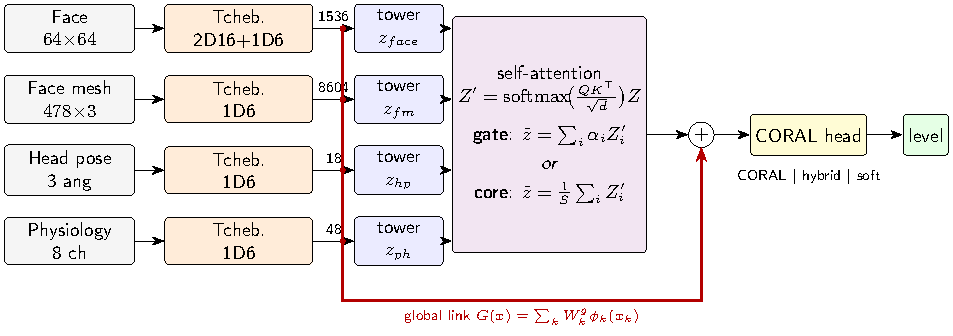
\includegraphics[width=0.72\textwidth]{fig_arch.pdf}
\caption{gTAO-Net. Fixed Tchebichef front-ends $\phi_k$ feed one tower per stream; the tower outputs are fused by a gate or by mean pooling (core); an optional linear global link connects the inputs to the head; a CORAL head is trained with one of three objectives.}
\label{fig:arch}
\end{figure*}

\subsection{Front-ends and towers}
Each stream is a short per-frame sequence. Frames of the image stream are converted to grey $64\times64$ images and projected on the two-dimensional Tchebichef basis of order 16~\cite{mukundan2001tchebichef}. Every image coefficient, landmark coordinate, angle and physiological channel is then projected in time on the one-dimensional basis of order 6. This yields fixed vectors $\phi_k$ of 1{,}536 (frame), 8{,}604 (mesh), 18 (pose) and 48 (physiology) dimensions, which are computed once and cached; no front-end parameter is learned. Our earlier benchmark used Tchebichef coefficients for the face image only~\cite{makhkhas2026ordinal}; here one transform family serves all four modalities, so adding a stream requires choosing a moment order rather than training an encoder. Each tower computes $z_k=\mathrm{LN}(W_2\,\mathrm{GELU}(W_1\phi_k))\in\mathbb{R}^{64}$, with a hidden size of 128 and layer normalisation (LN). A single-stream baseline consists of one tower followed by the head.

\subsection{Fusion}
The stacked tower outputs $Z$ pass through one self-attention step with bias-free query and key projections, $Z'=\mathrm{softmax}(QK^\top/\sqrt{d})Z$. The \emph{gate}, in the spirit of gated multimodal units~\cite{arevalo2017gated}, maps $Z'$ through a two-layer perceptron $g$ to weights $\alpha=\mathrm{softmax}(g(\mathrm{vec}\,Z'))$ and returns $\tilde z=\sum_i\alpha_iZ'_i$; these weights allow it to discard a stream. The \emph{core} variant, following CORE-Net~\cite{tran2026ordinal}, returns the mean $\tilde z=S^{-1}\sum_iZ'_i$ and cannot discard a stream. Following ModDrop~\cite{neverova2016moddrop}, modality dropout removes streams at random during training. Our variant zeroes each tower output with probability 0.2, independently per sample and stream and without rescaling, whereas ModDrop zeroes the inputs of pre-trained modality networks; the global link receives the unmasked inputs.

\subsection{Global link and objectives}
The global link $G(x)=\sum_kW^{g}_k\phi_k(x_k)$ is linear and bias-free. Structurally it is a projection shortcut~\cite{he2016deep} from the inputs to the head. The CORAL head~\cite{cao2020coral} computes $K-1$ logits $\ell_k=w^\top u+b_k$ with shared weights and one bias per threshold, where $u=\tilde z+G(x)$. Three objectives are compared.
\begin{itemize}
\item \textbf{CORAL}: a binary cross-entropy between $\sigma(\ell_k)$ and $\mathbf{1}[y>k]$.
\item \textbf{Hybrid}: inspired by CORE-Net~\cite{tran2026ordinal}, a cross-entropy on the implied class probabilities, plus 0.5 times the CORAL loss, plus 0.1 times a cross-entropy to a neighbour-smoothed target (0.7 on the true class and 0.15 on each neighbour, renormalised at the extremes). Unlike CORE-Net, it has no earth mover's term.
\item \textbf{Soft}: a binary cross-entropy against $t_k=1-\sum_{j\le k}\bar p_j$, the fraction of raters who voted above threshold $k$.
\end{itemize}

\noindent\textbf{Proposition.} If $\bar p$ is one-hot at $y$, then $t_k=\mathbf{1}[y>k]$ and the soft objective equals CORAL.

This is the ordinal counterpart of the observation that single-label learning is a special case of label distribution learning~\cite{geng2016ldl}. It has two consequences. On DAiSEE and EngageNet, where we use one label per sample, soft and CORAL are identical (confirmed bit-identical in the logs). On DIPSER, any difference between them arises from rater disagreement alone.

\section{Protocol}
\label{sec:protocol}

\subsection{Factorial design on the slice}
On the DIPSER slice we cross fusion $\in\{$gate, core$\}$, link $\in\{$on, off$\}$, dropout $\in\{$on, off$\}$ and objective $\in\{$CORAL, hybrid, soft$\}$. This gives 24 fusion configurations, to which we add eight single-stream baselines (four streams, CORAL and soft objectives) and one permuted-label control. With five folds and three seeds this amounts to 495 fits. The control is core fusion with link and dropout on and the CORAL objective, trained on labels permuted across the population; it is required to satisfy $|\mathrm{QWK}|\le0.10$. DAiSEE uses the same 24 configurations and three single-stream baselines (16 distinct fusion models, since soft and CORAL are identical). Because of the time limit of the computing platform, EngageNet uses a reduced set of configurations: three single streams, gate and core fusion with link on and dropout off, and the control (90 fits).

\subsection{Splits}
The main protocol (P2) is a five-fold cross-validation in which no grouping unit appears in both the training and the test fold; QWK is computed on the pooled out-of-fold predictions. On the slice the grouping unit is the student-session. The three students who have complete windows in both sessions may therefore contribute one session to training and the other to testing (5--20\% of the scored windows, depending on the seed); Section~\ref{sec:threats} reports a re-evaluation on person-disjoint windows. On the full release, folds group students, and a second protocol holds out one of the three class groups in turn (leave-one-class-out). For DAiSEE, protocol P1 trains on the official training subjects that do not appear in Validation and tests on Validation (1{,}429 clips); P1-Test retrains the best P1 single-stream and fusion models, selected on Validation, on Train and Validation, and scores them once on Test.

\subsection{Training}
Models are trained with Adam~\cite{kingma2015adam} (learning rate $3\times10^{-3}$, batch size 32, gradient clipping at 1.0) for at most 40 epochs, with early stopping after eight epochs without improvement and not before epoch 9. Epoch selection is nested: 20\% of the subjects of the training fold form an inner validation set, and the checkpoint with the best inner QWK is applied once to the outer fold, which avoids the selection bias of choosing the epoch on the scored fold~\cite{cawley2010overfitting}. A seed fixes the folds, the inner split, the initialisation and the sample order.

\subsection{Statistics}
On the slice, a factorial contrast compares matched configurations that differ in a single factor, with a two-sided Wilcoxon signed-rank test~\cite{wilcoxon1945} on configuration-level means (12 pairs for link, gate and dropout; 8 for the objectives); per-seed tests are reported as secondary. Values written $a\pm b$ are the mean and the standard deviation over three seeds. On the full release, headline values carry 95\% confidence intervals from a bootstrap over students, differences are paired on the same students, and families of related tests are corrected with the Holm procedure. The majority predictor (QWK $=0$) is the reference throughout.

\subsection{Predefined criteria and record of the study}
For the full release, the success criterion of each experiment was written in a dated analysis plan before the corresponding run; the plan, with its amendments, is part of the released material. One experiment, the hyper-parameter search of Section~\ref{sec:fc-limits}, had no predefined criterion and is labelled exploratory. Every reported number is produced by a notebook on a public computing platform (Kaggle), and a separate notebook recomputes the statistics from the stored outputs.

\section{Results on the DIPSER slice and transfer}
\label{sec:results}

\subsection{Fusion versus the best single stream (Q1)}
Fig.~\ref{fig:slice} shows the 33 configurations of the slice, and Supplementary Table~S1 lists them. The best single stream is the face mesh trained with the soft target (QWK $0.256\pm0.068$). The best fusion (gate, link on, dropout off, soft target) reaches $0.124\pm0.071$ and the best core fusion $0.113\pm0.073$. On identical folds, the best fusion falls short of the best single stream by $0.327$, $0.046$ and $0.021$ for the three seeds (mean $0.131$), so the size of the mean gap is driven by one seed. Only 1 of the 72 seed-level fusion results exceeds the best single stream of the same seed, and 14 of the 24 configurations score at or below zero.

Among the single streams, only the mesh carries signal on the slice (QWK $0.256$, against $0.003$ for the image stream, $0.002$ for physiology and $0.002$ for head pose, each with its better objective). The permuted-label control stays at $0.009\pm0.018$. Decision-level voting over the four single-stream predictions performs no better than feature-level fusion ($0.011\pm0.047$ and $0.006\pm0.028$ for streams trained with the soft and the CORAL objective).

\begin{figure}[!t]
\centering
\includegraphics[width=\columnwidth]{figures/fig_slice_grid.pdf}
\caption{DIPSER slice (1{,}566 complete windows, folds grouped by student-session). Each point is one configuration: pooled out-of-fold QWK, mean over three seeds; bars show the standard deviation over seeds. The dashed line marks the best single stream.}
\label{fig:slice}
\end{figure}

\subsection{Gate, global link and dropout (Q2, Q3)}
Table~\ref{tab:contrasts} reports the paired contrasts. The gate ends one-hot (weight $\ge0.98$ on one stream) in 108 of the 180 gated fits (60\%), and it selects the mesh stream, the only informative one, in 41 of them. Gate and core fusion do not differ significantly (gate better in 7 of 12 pairs, median difference $-0.009$, $p=0.68$); the same holds on DAiSEE ($p=0.46$ under P1 and $0.95$ under P2).

The global link improves QWK on the slice in 10 of 12 pairs (median $+0.076$, $p=0.002$). At initialisation it makes the gradient that reaches the first tower layers 12 to 132 times larger; these probes use a single seed and fold and do not establish the mechanism. On DAiSEE the effect is reversed: the link improves 0 of 8 pairs under P1 and 1 of 8 under P2 (median $-0.046$ and $-0.024$; $p=0.008$ and $0.016$). A possible explanation is that the link gives the head direct access to high-dimensional inputs that carry little signal on that dataset; we did not test it. Modality dropout has no reliable effect (better in 8 of 12 pairs, median $-0.016$, $p=0.62$).

\begin{table*}[!t]
\centering
\caption{Paired contrasts between configurations that differ in one factor. Wins: pairs in which the first level has the higher mean QWK. Med./Mean $\Delta$: median and mean per-seed QWK differences. $p_{\text{cfg}}$: Wilcoxon signed-rank test on configuration-level means (primary); $p_{\text{seed}}$: on per-seed differences (secondary). Values are not corrected for multiple comparisons; see Section~\ref{sec:threats}.}
\label{tab:contrasts}
\small
\setlength{\tabcolsep}{3pt}
\begin{tabular}{llccccc}
\toprule
Contrast & Data & Wins & Med. $\Delta$ & Mean $\Delta$ & $p_{\text{cfg}}$ & $p_{\text{seed}}$ \\
\midrule
\csname @@input\endcsname tables/contrasts.tex
\bottomrule
\end{tabular}
\end{table*}

\subsection{Ordinal objectives (Q4)}
In the fusion configurations the soft target outperforms CORAL in 7 of 8 pairs (median $+0.062$, $p=0.023$) and the hybrid objective in 7 of 8 ($+0.117$, $p=0.016$). By the proposition of Section~\ref{sec:instrument}, a difference between soft and CORAL can only come from rater disagreement. The evidence is nevertheless weak. After a Holm correction over the slice contrasts only the link remains significant ($p=0.012$; soft against CORAL, $p=0.070$), on person-disjoint windows the soft target wins 6 of 8 pairs without significance ($p=0.078$), and for single streams it wins 2 of 4 pairs. For the mesh stream it raises QWK from $0.092$ to $0.256$, and for the image stream from $-0.163$ to $0.003$.

Zeroing one stream at inference harms both fusion types, most strongly the mesh stream for the gate ($-0.129$) and the image stream for core fusion ($-0.111$). On the high level, which has seven windows, recall is 0.00 for the best single stream and 0.19 for the best fusion, which over-predicts this level; 81--99\% of the errors are one level off.

\subsection{Transfer to DAiSEE and EngageNet (Q5)}
Table~\ref{tab:transfer} gives the transfer results. Fusion yields no meaningful gain over the best single stream on DAiSEE ($+0.010$ under P2 and $-0.001$ under P1), and it trails it on the EngageNet frames (gate $0.170$ against mesh $0.366$). The permuted controls remain near zero ($0.024$ and $0.035$). The informative stream differs between datasets: the mesh leads on DIPSER and on EngageNet, whereas on DAiSEE the image stream (P1, $0.093$) and the head pose (P2, $0.050$) lead, and no configuration exceeds QWK $0.10$.

\begin{table*}[!t]
\centering
\caption{Transfer: pooled QWK (mean $\pm$ s.d. over three seeds). $\Delta$: best fusion minus best single stream. Perm.: permuted-label control. $^\dagger$Reduced set of configurations, frame-level samples, P2 only.}
\label{tab:transfer}
\small
\setlength{\tabcolsep}{2.5pt}
\begin{tabular}{lcccccc}
\toprule
Setting & Image & Mesh & Pose & Best fusion & $\Delta$ & Perm. \\
\midrule
\csname @@input\endcsname tables/transfer.tex
\bottomrule
\end{tabular}
\end{table*}

\textbf{Position with respect to published DAiSEE results.} Table~\ref{tab:comparison} places the instrument beside published systems on the official test set. On that set, the best single stream (image stream, CORAL, selected on Validation) obtains QWK $0.043\pm0.013$ at 50.4\% accuracy and the best fusion $0.044\pm0.018$, while the majority predictor reaches 51.8\% on the clips we score. Published studies report accuracy and no QWK, but three of them print a test confusion matrix, from which we derive QWK values between \pubResTcnQwk{} and \pubOrdTcnQwk. With a training-free moment front-end and six frames per clip, the instrument is therefore far below systems that use learned spatio-temporal features on DAiSEE, and its DAiSEE results should be read only as a within-instrument comparison of fusion against single streams. The table also shows the limits of accuracy on this dataset: the lowest level has four test clips, so that its recall can only be 0 or a multiple of 0.25, and the system with the highest accuracy among those with a printed matrix has a recall of \pubOrdTcnRecOne{} on the second level (84 clips).

\begin{table}[!t]
\centering
\caption{DAiSEE, four classes, official test set. Published rows: single reported runs on 1{,}784 clips (majority rate \pubMajority\%). Our rows: mean over three seeds on the 1{,}638 clips with all streams (P1-Test). Rec.\,0 and Rec.\,1: recall of the two lowest levels (4 and 84 clips in the full test set). $^\ast$Derived by us from the published confusion matrix; n.r.: not reported and not derivable.}
\label{tab:comparison}
\footnotesize
\setlength{\tabcolsep}{2pt}
\begin{tabular}{lcccc}
\toprule
Method & Acc.\,\% & Rec.\,0 & Rec.\,1 & QWK \\
\midrule
DFSTN~\cite{liao2021dfstn} & 58.84 & n.r. & n.r. & n.r. \\
ResNet+TCN~\cite{abedi2021resnettcn} & 63.9 & 0.00$^\ast$ & \pubResTcnRecOne$^\ast$ & \pubResTcnQwk$^\ast$ \\
Ordinal TCN~\cite{abedi2024affectordinal} & 67.4 & 0.25$^\ast$ & \pubOrdTcnRecOne$^\ast$ & \pubOrdTcnQwk$^\ast$ \\
Contrastive ordinal~\cite{abedi2025supervised} & 67.32 & 0.00 & \pubContrastiveRecOne & \pubContrastiveQwk$^\ast$ \\
ViBED-Net (preprint)~\cite{gothwal2025vibednet} & 73.43 & 0.25 & 0.79 & n.r. \\
\midrule
Majority (1{,}638 clips) & 51.8 & 0.00 & 0.00 & 0.00 \\
gTAO-Net, best single stream & 50.4 & 0.00 & 0.02 & $0.043\pm0.013$ \\
gTAO-Net, best fusion & 50.2 & 0.00 & 0.01 & $0.044\pm0.018$ \\
\bottomrule
\end{tabular}
\end{table}

\textbf{Computational cost.} The 495 fits of the slice train in 24 minutes on a Kaggle GPU and in an estimated 15--18 minutes on a laptop CPU; the GPU brings no speed-up for models of 1.12 to 2.07 million parameters (Supplementary Table~S2). Tchebichef encoding takes 0.6\,ms per window.

\section{Results on the full DIPSER release (Q6)}
\label{sec:fullcorpus}

On the full release, folds group students unless a class is held out, and each success criterion was fixed before the run unless the experiment is marked exploratory.

\subsection{Replication of the fusion result}
\label{sec:fc-fusion}
The factorial grid was rerun with inputs standardised on the training fold, student-grouped folds and three seeds. The fusion result is replicated (Fig.~\ref{fig:full}): \fcFusionsAbove{} fusion configurations exceed the best single stream, which is again the face mesh (QWK \fcBestSingleQWK, 95\% CI \fcBestSingleCI). The best fusion obtains \fcBestFusionQWK, and the paired difference is \fcFusionDiff{} \fcFusionDiffCI{} ($p=\fcFusionP$). The data are thus compatible with a small difference in either direction, but not with a fusion gain larger than about 0.02.

All streams are considerably weaker than on the slice. On the slice, 59\% of the label variance lies between the 20 students, so that a model can score by recognising which students tend to be rated as attentive; this is no longer the case with \fcPersons{} students (Section~\ref{sec:fc-labels}). Two further measurements indicate what the models capture. First, the agreement with changes \emph{within} a student-session is small (correlation $\le\fcWithinSessionMax$ for every stream). Second, no stream significantly outperforms a control model that is trained on the label of a \emph{classmate} at the same moment (closest: the \fcClassmateStream{} stream, $p=\fcClassmateP$; dashed line in Fig.~\ref{fig:full}). The streams of a student therefore carry mainly information about what the class is doing, and little that is specific to the student.

\begin{figure}[!t]
\centering
\includegraphics[width=\columnwidth]{figures/fig_full_release.pdf}
\caption{Full DIPSER release, held-out students. QWK of the best configuration of each single stream and of the best fusion, with 95\% bootstrap intervals over students. Grey bars: label-only references that use the labels of the other students (not deployable). Dashed line: highest QWK of the classmate-label controls.}
\label{fig:full}
\end{figure}

\subsection{Structure of the labels}
\label{sec:fc-labels}
Of the label variance, \fcSharePerson\% lies between students, \fcShareClass\% between class sessions and \fcShareSession\% between student-sessions. In this dataset the rated attention is thus mainly a property of a lesson, and of a student within that lesson, rather than a stable trait of the student; the nine sessions of a group are nine different activities. Two label-only references quantify this structure. They use no sensor, and they cannot be deployed because they read the labels of other students. The mean label of the other students in the same class session yields QWK \fcExpPrior, and the labels of the other students at the same 4-s moment yield \fcMomentPrior. Both are about three times the best sensor model (Fig.~\ref{fig:full}).

\subsection{Attempts to improve the sensor model}
\label{sec:fc-limits}
Table~\ref{tab:fc-tests} summarises the attempts; every comparison is paired on the same students.

\textbf{Search and higher-order moments.} A Bayesian search (tree-structured Parzen estimator) over the streams, the moment orders, the model family (multilayer perceptron or gradient-boosted trees), the model size, the learning rate, the class weights and the head was evaluated on a fixed split with 13 held-out test students, scored once with three seeds. It reaches \fcSearchPaperAcc\% test accuracy against a majority rate of \fcSearchMajority\%. Moments re-extracted at higher orders ($24\times24$ in space, 12 in time) give \fcSearchRichAcc\%, a difference that is not significant, and the search itself selects low orders (6--8 in space, 5--7 in time).

\textbf{Face crop and moment families.}
\label{sec:fc-crop}
Because the image stream is the whole webcam frame, we constructed a face crop from the per-frame face box of the DIPSER metadata (square, 10\% margin). Frames without a detected face become blank images, so that the visibility of the face is itself encoded. The crop was described with five discrete orthogonal moment families: Tchebichef, Hahn ($\alpha=\beta=4$) and Krawtchouk centred on the face, on the eyes and on the mouth. Unlike Tchebichef moments, Hahn and Krawtchouk moments are local and concentrate on a region of the image. A self-test confirmed that the whole-frame Tchebichef moments recomputed by the new pipeline equal the original features in all 35{,}374 comparable windows. The crop raises accuracy by \fcCropAccGain{} points \fcCropAccCI{} over the whole frame, but it does not significantly change QWK. No family outperforms Tchebichef under the predefined rule, which required a Holm-corrected gain in both an accuracy-tuned and a QWK-tuned search; the best family, Hahn, gains $+0.036$ in the latter (Holm $p=0.13$) and $+0.010$ in the former.

\textbf{Temporal and class context.} Because the raters mark change points, consecutive windows usually share a label. A causal recurrent model (GRU) that reads the preceding windows of the student nevertheless leaves QWK unchanged (\fcCtxNoneQWK{} for isolated windows, \fcCtxGruQWK{} with the past, and \fcCtxBiQWK{} for an offline bidirectional model). Adding the sensor features of the other students at the same moment, without their labels, does not significantly improve QWK on a class unseen during training (\fcLogoOwnQWK{} to \fcLogoClassQWK).

\textbf{Pretrained face encoders.} To test whether the moment front-end is the limiting factor, we added frozen pretrained encoders of the face crop to the sensor features (mean and standard deviation of the embeddings of up to eight crops per window): ResNet-18~\cite{he2016deep}, DINOv2~\cite{oquab2024dinov2} and an expression network trained for emotion and engagement~\cite{savchenko2022hsemotion}. On a held-out class the sensor features give \fcEncBaseAcc\% accuracy and QWK \fcEncBaseQWK; adding an encoder gives QWK \fcEncResQWK, \fcEncDinoQWK{} and \fcEncExprQWK{} respectively, none significantly different. The third encoder was added after the results of the first two were known.

\begin{table*}[!t]
\centering
\caption{Attempts to improve performance on the full release. $\Delta$QWK: second condition minus first, paired on the same students (bootstrap over students, 95\% CI); two-sided $p$, Holm-adjusted within the moment families and within the encoders. Phase: label of the experiment in the released plan. Rule: pre-decl., criterion fixed before the run; explor., no predefined criterion.}
\label{tab:fc-tests}
\small
\setlength{\tabcolsep}{2.5pt}
\begin{tabular}{lcccccc}
\toprule
Comparison & Phase & Rule & $\Delta$QWK & 95\% CI & $p$ & Improves \\
\midrule
\csname @@input\endcsname tables/fullcorpus_tests.tex
\bottomrule
\end{tabular}
\end{table*}

\subsection{Tracking with sparse label probes}
\label{sec:fc-probe}
Since sensors alone fail, we tested a different task, in which some labels are available at test time. The consensus label of a student is revealed at a probe every 32\,s, 1\,min or 2.5\,min, and the windows in between are predicted causally. The model reads the sensors of the current window and of the last probe window, the labels of the last two probes and the time since the last probe; it never reads a later label or the label of another student. Evaluation is on a held-out class, with gradient-boosted trees, three seeds and all \fcWindows{} windows (majority rate \fcMajorityAll\%); the model settings and the decision rules were fixed in advance.

Table~\ref{tab:fc-probe} and Fig.~\ref{fig:probe} compare three predictors: repeating the last probe (persistence), a model of the probe labels alone, and the same model with sensors. With a probe every 32\,s the full model reaches \fcProbeHalfAcc\% accuracy and QWK \fcProbeHalfQWK, and with one probe per minute \fcProbeOneAcc\% and \fcProbeOneQWK, against \fcSensorsOnlyAcc\% and \fcSensorsOnlyQWK{} for sensors alone. Persistence, however, already obtains \fcPersistHalfAcc\% and \fcPersistHalfQWK{} (\fcPersistOneAcc\% and \fcPersistOneQWK{} per minute). The sensors add between 1 and 3 points of accuracy, with confidence intervals that exclude zero, and no QWK. This is consistent with a report on self-rated attention in video learning, in which carrying the last rating forward gives a lower error than sensor models when forecasting the next ratings~\cite{leng2026edugage}.

The probe above is the consensus label. With the self-report of the student as the probe and the expert labellers as the target, persistence gives only \fcSelfPersistHalfAcc\% accuracy and QWK \fcSelfPersistHalfQWK{} at 32\,s, because the self-reports agree poorly with the labellers (QWK \fcSelfExtQWK). The self-reports of DIPSER are given retrospectively~\cite{marquezcarpintero2025dipser}, which may contribute to this disagreement. The tracking result therefore requires probes of observer quality.

\begin{figure}[!t]
\centering
\includegraphics[width=\columnwidth]{figures/fig_probe.pdf}
\caption{Sparse-probe tracking on a held-out class: accuracy on the windows between probes as a function of the probe interval (three seeds). The gap between the two upper curves is the contribution of the sensors.}
\label{fig:probe}
\end{figure}

\begin{table*}[!t]
\centering
\caption{Sparse-probe tracking on a held-out class (accuracy\,\% / QWK on the windows between probes, three seeds). Gain: probe + sensors minus persistence, bootstrap over students, 95\% CI.}
\label{tab:fc-probe}
\small
\setlength{\tabcolsep}{3pt}
\begin{tabular}{lccccc}
\toprule
Probe every & Persistence & Probe model & Probe + sensors & Acc.\ gain (points) & QWK gain \\
\midrule
\csname @@input\endcsname tables/fullcorpus_probe.tex
\bottomrule
\end{tabular}
\end{table*}

\subsection{Effect of the evaluation protocol}
\label{sec:fc-protocol}
Table~\ref{tab:fc-protocol} and Fig.~\ref{fig:protocol} report two experiments, each of which keeps the model fixed and changes only what the test set shares with the training set.

In the first, model A is evaluated on random windows and on held-out students. With random windows, the windows of a student fall on both sides of the split, often seconds apart, and the model obtains \fcLeakRandAcc\% accuracy and QWK \fcLeakRandQWK. With whole students held out it obtains \fcLeakPersonAcc\% and \fcLeakPersonQWK{} (majority rate \fcMajority\%).

In the second, model B is evaluated on held-out students and on a held-out class. Holding out a class lowers QWK from \fcPgOwnQWK{} to \fcLogoOwnQWK{} (paired difference for seed 0: \fcLogoDrop{} \fcLogoDropCI), which indicates that part of what is learned is specific to the lessons seen in training. The effect is largest when class features are used (model B$'$). With students held out, these features appear to raise QWK from \fcPgOwnQWK{} to \fcPgClassQWK{} (\fcLeakClassDiff{} \fcLeakClassCI): the labels of the classmates at the same moment are in the training set, and the class features allow the model to retrieve them. On an unseen class this gain disappears.

Across the splits that hold out students or classes, accuracy remains within a few points of the majority rate (\fcLogoOwnAcc--\fcLeakPersonAcc\% against \fcMajority\%), whereas QWK decreases four-fold from random windows to a held-out class.

\begin{figure}[!t]
\centering
\includegraphics[width=\columnwidth]{figures/fig_protocol.pdf}
\caption{The same models under different splits (full release, complete windows). A: model of the hyper-parameter search; B: window-level perceptron on all streams including the face crop; B$'$: B with the sensor features of the classmates. Dashed line: majority accuracy.}
\label{fig:protocol}
\end{figure}

\begin{table*}[!t]
\centering
\caption{The same model under different splits (full release, complete windows, pooled out-of-fold predictions, majority accuracy \fcMajority\%). A: model of the hyper-parameter search (three seeds); B: window-level perceptron on all streams including the face crop (three seeds; student-grouped: one seed); B$'$: B with the sensor features of the classmates.}
\label{tab:fc-protocol}
\small
\setlength{\tabcolsep}{3pt}
\begin{tabular}{lllcc}
\toprule
Model & Split & Shared with the training set & Acc.\,\% & QWK \\
\midrule
\csname @@input\endcsname tables/fullcorpus_protocol.tex
\bottomrule
\end{tabular}
\end{table*}

\section{Discussion}
\label{sec:discussion}

Fusion yields no meaningful gain over the best single stream on any of the three datasets or on the full DIPSER release (at most $+0.010$ QWK, on DAiSEE). This agrees with accounts of multimodal failure~\cite{wang2020makes,peng2022balanced}: the gate collapses to one stream chosen by the optimisation rather than by how informative it is, and mean pooling weakens the single informative stream with uninformative ones. The components that help concern optimisation and supervision rather than fusion: the global link gives the head direct access to all inputs, and the soft target exploits the rater distribution and yields the best single model on the slice.

The full release changes the interpretation of the slice. On the slice, models appeared useful because they ranked 20 students; with 57 students, labels vary mainly between lessons, and the sensor signal is largely shared by the class. Neither richer or local moments, nor a face crop, nor pretrained face encoders, nor temporal or class context finds a student-specific signal, so the limitation lies in how little the per-student streams convey about labels that vary with the lesson, rather than in the encoder.  Each relaxation of the split introduces a leak: the same student a few seconds apart, classmates in the same lesson, and classmates' labels retrieved through class features. Accuracy hides all three, because it remains close to the majority rate.

\textbf{Recommendations.} (1) Report the best single-stream baseline under the same protocol as any fusion model. (2) With multiple raters, train on the vote distribution rather than the majority vote. (3) Interpret one-hot gates as stream selection, not fusion. (4) Do not transfer components across datasets without testing them, since the link helps on DIPSER but harms on DAiSEE. (5) For imbalanced ordinal labels, base conclusions on QWK and report accuracy together with the majority rate. (6) For claims about classrooms, hold out whole classes, since person-grouped folds still share lessons and, with class-level features, leak classmates' labels. (7) Report label-only references alongside the majority class; here, the other students of the same lesson give QWK \fcExpPrior. (8) When earlier labels of the same student are available, report label persistence~\cite{demasi2017meaningless}.

\subsection{Threats to validity}
\label{sec:threats}
On the slice, folds group student-sessions rather than persons; re-evaluating every run on person-disjoint windows leaves the main findings unchanged (no fusion above the best stream; gate versus core $p=0.79$; link 10 of 12 pairs, $p=0.021$; best stream $0.213$, best fusion $0.109$), but the soft-target gain is no longer significant ($p=0.078$). Nested selection removes selection bias but trains on 80\% of the fold subjects, so absolute values are not comparable with the earlier non-nested version~\cite{cawley2010overfitting}. Only complete windows are used, which removes 47\% of the slice and 19\% of the full release. The slice contains seven high-attention windows, the mean fusion gap is driven by one seed, and the gradient probes use a single seed and fold. The face stream of the slice experiments is the whole webcam frame; Section~\ref{sec:fc-crop} tests a true crop. The full-release attempts used fixed model families (MLP, gradient-boosted trees, GRU); the face encoders were frozen, so we conclude that moment features, pretrained embeddings and context do not help, not that an encoder fine-tuned on classroom data could not. Leave-one-class-out uses only three folds (20, 21 and 16 students), and its estimates are correspondingly noisy. The DAiSEE comparison uses only clips with all streams, and the EngageNet results rely on a subset of configurations and on frame-level samples.

\section{Conclusion}
\label{sec:conclusion}

Using one instrumented model and a nested protocol, we find that multimodal fusion does not improve classroom attention estimation. On a DIPSER slice, no fusion configuration exceeds face mesh with the soft target ($0.256$ against $0.124$), the gate does not differ from mean pooling, and only the input-to-head link and the soft target help; fusion also brings no gain on DAiSEE and EngageNet. On the full DIPSER release the fusion result replicates, but the per-student signal is weak and largely shared by the class, and hyper-parameter search, richer and local moments, a face crop, frozen pretrained face encoders, and temporal and class context fail to improve it. The evaluation split has a larger effect than any modelling choice: one model obtains QWK \fcLeakRandQWK{} on random windows, \fcLeakPersonQWK{} on held-out students and \fcLogoOwnQWK{} on a held-out class, with accuracy near the \fcMajority\% majority rate. Sparse probes of the raters' label raise accuracy above 70\%, but label persistence explains almost all of this gain, and self-report probes do not reproduce it. Classroom attention systems should therefore be evaluated on held-out classes, with QWK and label-only references. Future work will fine-tune face encoders and evaluate them on held-out classes.

\section*{Data and code availability}
DIPSER~\cite{marquezcarpintero2025dipser} is distributed by its authors on request under a CC-BY licence; DAiSEE~\cite{gupta2016daisee} and EngageNet~\cite{singh2023engagenet} are available from their authors. We do not redistribute any recording. The repository \url{https://github.com/mks-zakaria/gtao-net} contains the per-seed results, the out-of-fold predictions of the slice and transfer experiments, the summaries and logs of the full-release experiments, the source of every notebook, the analysis plan with its predefined criteria, the scripts that regenerate every table and figure, and a verification script that recomputes the reported numbers of the slice and transfer experiments from the raw predictions. The training notebooks of the slice and transfer experiments are public: DIPSER \url{https://www.kaggle.com/code/zakariamakhas/gtao-net-dipser-grid-v2-nested-early-stopping}, DAiSEE \url{https://www.kaggle.com/code/zakariamakhas/gtao-net-daisee-v2-nested-early-stopping} and EngageNet \url{https://www.kaggle.com/code/zakariamakhas/gtao-net-engagenet-v2-nested-early-stopping}; the EngageNet frames are the Kaggle datasets \texttt{laavanayadhawan/engagenet-personalization} and \texttt{laavanayadhawan/openface-engagenet}. \pending{Full-release notebooks: list the public URLs once their visibility is changed (see the repository README for the list).}

\section*{Ethics statement}
This study uses existing datasets only. The authors of DIPSER report approval by the ethics committee of their university and signed informed consent of all participants~\cite{marquezcarpintero2025dipser}. No new data were collected from human participants, and no image of a participant is reproduced in this article.

\section*{Conflict of interest}
The authors declare no competing interests.

\section*{Acknowledgment}
The authors used a generative AI assistant (Anthropic Claude) during the preparation of this manuscript. It was used to draft and revise prose in all sections and to assist in writing the analysis and figure-generation code. All experiments were executed by the authors, and all reported values were computed by running that code. No AI system contributed analysis results or figures. The authors reviewed all content and take full responsibility for it.


\bibliographystyle{IEEEtran}
\bibliography{references}

\begin{IEEEbiographynophoto}{Zakaria Makhkhas}
is a doctoral researcher with the Laboratory of Information Modelling and Communication Systems, Faculty of Sciences, University Ibn Tofail, K\'enitra, Morocco (ORCID 0009-0005-9002-8860). His doctoral research concerns multimodal machine learning for the recognition of student attention and engagement in the classroom, with a focus on discrete orthogonal moments, ordinal classification and evaluation protocols. \pending{Degrees with institution and year, and photograph, to be added by the author.}
\end{IEEEbiographynophoto}
\begin{IEEEbiographynophoto}{Amal Rifai}
is with the Team of Research in Engineering of Computing Environment for Human Learning, Regional Center for the Professions of Education and Training (RCPET), Rabat, Morocco. Her research interests include computing environments for human learning, the modelling of learning scenarios, computer-based and personalised tutoring, and data-driven decision support in education. \pending{Degrees with institution and year, current position, and photograph, to be added by the author.}
\end{IEEEbiographynophoto}
\begin{IEEEbiographynophoto}{Abdelalim Sadiq}
is with the Laboratory of Information Modelling and Communication Systems, Faculty of Sciences, University Ibn Tofail, K\'enitra, Morocco. His research interests include the detection of student attention in the classroom from video, facial emotion recognition and image analysis. \pending{Degrees with institution and year, current position, and photograph, to be added by the author.}
\end{IEEEbiographynophoto}
\EOD
\end{document}
